\documentclass[14pt, a4paper]{article}
\usepackage{minitoc}
\usepackage[left=3.00cm, right=2.5cm, top=2.00cm, bottom=2.00cm]{geometry}
\usepackage{amsmath}
\usepackage{amssymb}
\usepackage{amsthm}
\usepackage{mathtools}
\usepackage{graphicx}
%\usepackage{algpseudocode}
%\usepackage{algorithm}
\usepackage[ruled,vlined,linesnumbered]{algorithm2e}
\usepackage{blindtext}
\usepackage{setspace}
\usepackage[utf8]{inputenc}
\usepackage[utf8]{vietnam}
\usepackage[center]{caption}
\usepackage[shortlabels]{enumitem}
\usepackage{fancyhdr} % header, footer
\usepackage{hyperref} % loại bỏ border với mục lục và công thức
\usepackage[nonumberlist, nopostdot, nogroupskip]{glossaries}
\usepackage{glossary-superragged}
\usepackage{tikz,tkz-tab}
\usepackage{pythonhighlight}
\setglossarystyle{superraggedheaderborder}
\pagestyle{fancy}
%\usepackage[style=numeric,sortcites]{biblatex}
%\addbibresource{ref.bib}
%\usepackage[numbers]{natbib}
\usepackage{indentfirst}
\usepackage[natbib,backend=biber,style=ieee, sorting=ynt]{biblatex}

\usepackage{caption}
\usepackage{subcaption}

\bibliography{ref.bib}

\graphicspath{{./figures/}}

\fancyhf{}
%\rhead{\textbf{Môn học: Các phương pháp thống kê hiện đại trong nghiên cứu Xã hội học}}
\lhead{\textbf{GVHD: TS. Trịnh Quốc Anh}}
\rfoot{\thepage}
\lfoot{\textbf{Học viên thực hiện: Nguyễn Chí Thanh - 21007925}}
\renewcommand{\headrulewidth}{0.4pt}
\renewcommand{\footrulewidth}{0.4pt}
%
%\numberwithin{equation}{section}
%\numberwithin{algorithm}{section}
%\numberwithin{figure}{section}
%
%\setlength{\parindent}{0.5cm}
%
%\setcounter{secnumdepth}{3} % Cho phép subsubsection trong report
%\setcounter{tocdepth}{3} % Chèn subsubsection vào bảng mục lục

%\newtheorem{dl}{Định lý}
%\newtheorem{md}{Mệnh đề}
%\newtheorem{bd}{Bổ đề}
%\newtheorem{dn}{Định nghĩa}
%\newtheorem{hq}{Hệ quả}

%\newtheorem{baitap}{Bài tập}
%\newtheorem*{loigiai}{Lời giải}

%\numberwithin{dl}{section}
%\numberwithin{md}{section}
%\numberwithin{bd}{section}
%\numberwithin{dn}{section}
%\numberwithin{hq}{section}

\setlength{\parindent}{0cm}

\newtheorem{dl}{Định lý}
\newtheoremstyle{sltheorem}
{}                % Space above
{}                % Space below
{\normalfont}        % Theorem body font % (default is "\upshape")
{}                % Indent amount
{\bfseries}       % Theorem head font % (default is \mdseries)
{.}               % Punctuation after theorem head % default: no punctuation
{ }               % Space after theorem head
{}                % Theorem head spec
\theoremstyle{sltheorem}
\newtheorem{baitap}{Bài tập}
\newtheoremstyle{soltheorem}
{}                % Space above
{}                % Space below
{\normalfont}        % Theorem body font % (default is "\upshape")
{}                % Indent amount
{\bfseries}       % Theorem head font % (default is \mdseries)
{.}               % Punctuation after theorem head % default: no punctuation
{\newline}               % Space after theorem head
{}                % Theorem head spec
\theoremstyle{soltheorem}
\newtheorem*{loigiai}{Lời giải}

\onehalfspacing

\begin{document}
\begin{titlepage}

    \newcommand{\HRule}{\rule{\linewidth}{0.5mm}} % Defines a new command for the horizontal lines, change thickness here

    \center % Center everything on the page

    %----------------------------------------------------------------------------------------
    %	HEADING SECTIONS
    %----------------------------------------------------------------------------------------
    \textsc{\LARGE Đại học Quốc Gia Hà Nội}\\[0.5cm]
    \textsc{\LARGE Trường đại học Khoa học tự nhiên}\\[0.5cm] % Name of your university/college
    \textsc{\LARGE Khoa Toán - Cơ - Tin học}\\[0.5cm]

    
\includegraphics[scale=0.2]{HUS-logo.jpg}\\[0.5cm]

    \textsc{\Large Chuyên ngành: Khoa học dữ liệu}\\[0.5cm] % Major heading such as course name


    %----------------------------------------------------------------------------------------
    %	TITLE SECTION
    %----------------------------------------------------------------------------------------

    \HRule \\[0.4cm]
    { \huge \bfseries Bài tập môn học}\\[0.4cm] % Title of your document
    \HRule \\[1.5cm]

    \textsc{\Large Môn học: Các phương pháp thống kê hiện đại \\ trong nghiên cứu Xã hội học}\\[1cm] % Minor heading such as course title


    \textsc{\Large Bài tập số 3}\\[1cm]


    %----------------------------------------------------------------------------------------
    %	AUTHOR SECTION
    %----------------------------------------------------------------------------------------
    \begin{minipage}{0.4\textwidth}
        \begin{flushleft} \large
        \emph{Giảng viên hướng dẫn:} \\
        TS. Trịnh Quốc Anh % Supervisor's Name
        \end{flushleft}
    \end{minipage}\\[0.5cm]

    \begin{minipage}{0.4\textwidth}
    \begin{flushleft} \large
    \emph{Học viên thực hiện:}\\
    Nguyễn Chí Thanh \\
    MSHV: 21007925 \\ % Your name
    Lớp: Khoa học dữ liệu - K4
    \end{flushleft}
    \end{minipage}


    % If you don't want a supervisor, uncomment the two lines below and remove the section above
    %\Large \emph{Author:}\\
    %John \textsc{Smith}\\[3cm] % Your name

    %----------------------------------------------------------------------------------------
    %	DATE SECTION
    %----------------------------------------------------------------------------------------

    % I don't want day because it is English
    % {\large \today}\\[2cm] % Date, change the \today to a set date if you want to be precise

    %----------------------------------------------------------------------------------------
    %	LOGO SECTION
    %----------------------------------------------------------------------------------------

    %\includegraphics{logo/rsz_3logo-khtn.png}\\[1cm] % Include a department/university logo - this will require the graphicx package

    %----------------------------------------------------------------------------------------

    \vfill % Fill the rest of the page with whitespace

\end{titlepage}

\nocite{*}

\newpage

\begin{baitap}
    Áp dụng các phương pháp Ridge, LASSO, và PCA cho dữ liệu Sonar.

    Hãy so sánh các kết quả thu được và biện luận để đưa ra mô hình phù hợp nhất.
\end{baitap}

\begin{loigiai}
    Hàm mất mát của mô hình logistic regression:
    \begin{equation*}
        \mathcal{L} = -\dfrac{1}{N}\sum_{i=1}^N (y_i \log \hat{y}_i + (1-y_i)\log(1-\hat{y}_i)) 
    \end{equation*}

    với $\hat{y}=p(y=1\vert \bold{x})=f(\bold{x}) = \sigma(w_0 + w_1 x_1 + w_2 x_2 + \dots w_n x_n) = \sigma(\bold{w}^T \bold{x})$ là kết quả đầu ra của mô hình logistic tương ứng với đầu vào $\bold{x}$.

    Hàm mất mát của phương pháp Ridge:

    \begin{equation*}
        \mathcal{L}_{\mathrm{Ridge}} = -\dfrac{1}{N}\sum_{i=1}^N (y_i \log \hat{y}_i + (1-y_i)\log(1-\hat{y}_i)) + \lambda \lVert \bold{w} \rVert_2^2
    \end{equation*}

    Hàm mất mát của phương pháp LASSO:

    \begin{equation*}
        \mathcal{L}_{\mathrm{Ridge}} = -\dfrac{1}{N}\sum_{i=1}^N (y_i \log \hat{y}_i + (1-y_i)\log(1-\hat{y}_i)) + \lambda \lVert \bold{w} \rVert_1
    \end{equation*}

    Để xây dựng mô hình, ta sẽ sử dụng các hướng sau:

        \begin{itemize}
            \item Mô hình bao gồm tất cả các biến (đặc trưng) từ tập dữ liệu.
            \item Mô hình bao gồm các đặc trưng được trích xuất từ thuật toán PCA giữa lại 95 \% thông tin.
            \item Mô hình gồm các biến được chọn từ hàm step() để lựa chọn mô hình trong ngôn ngữ R.
        \end{itemize}

    Dữ liệu trước khi đưa vào hàm step() trong R được tiền xử lý theo hai cách:

    \begin{itemize}
        \item Min max scaling (minmax)
        \item Standardize
    \end{itemize}

    Ta kiểm định các hệ số của mô hình forward sử dụng likelihood ratio test:

\begin{verbatim}
    anova(minmax_m.f, test="Chisq")
\end{verbatim}

    \begin{verbatim}
Df	Deviance	Resid. Df	Resid. Dev	Pr(>Chi)
<int>	<dbl>	<int>	<dbl>	<dbl>
NULL	NA	NA	207	287.40621	NA
V11	1	45.813415	206	241.59279	1.300698e-11
V47	1	19.278348	205	222.31444	1.129803e-05
V36	1	14.276700	204	208.03774	1.578062e-04
V45	1	11.188262	203	196.84948	8.231642e-04
V4	1	7.877562	202	188.97192	5.005192e-03
V15	1	7.147110	201	181.82481	7.508488e-03
V21	1	10.009874	200	171.81494	1.557032e-03
V51	1	5.049499	199	166.76544	2.463306e-02
V8	1	6.307759	198	160.45768	1.202107e-02
V49	1	4.305721	197	156.15196	3.798439e-02
V50	1	3.675029	196	152.47693	5.523328e-02
V1	1	4.399958	195	148.07697	3.593981e-02
V3	1	3.994465	194	144.08250	4.564995e-02
V52	1	4.131899	193	139.95061	4.208211e-02
V54	1	5.142063	192	134.80854	2.335288e-02
V23	1	5.266855	191	129.54169	2.173524e-02
V29	1	3.784617	190	125.75707	5.172573e-02
V31	1	5.069299	189	120.68777	2.435323e-02
V12	1	5.208250	188	115.47952	2.247995e-02
V30	1	3.796447	187	111.68307	5.136148e-02
V32	1	6.695459	186	104.98762	9.665880e-03
V53	1	3.503780	185	101.48384	6.122894e-02
V7	1	3.585955	184	97.89788	5.826991e-02
V16	1	4.186234	183	93.71165	4.075352e-02
V9	1	3.377209	182	90.33444	6.610391e-02
V26	1	3.287893	181	87.04654	6.979253e-02
V37	1	3.799709	180	83.24684	5.126148e-02
V34	1	2.558428	179	80.68841	1.097077e-01
V35	1	3.043974	178	77.64443	8.103731e-02
V38	1	2.682565	177	74.96187	1.014522e-01
V6	1	2.916942	176	72.04493	8.765385e-02
V40	1	2.279184	175	69.76574	1.311208e-01
V59	1	2.302910	174	67.46283	1.291319e-01
V19	1	2.118068	173	65.34476	1.455701e-01
V56	1	2.415767	172	62.92900	1.201192e-01
    \end{verbatim}

    \begin{verbatim}
anova(standardize_m.f, test="Chisq")
    \end{verbatim}

    \begin{verbatim}
Df	Deviance	Resid. Df	Resid. Dev	Pr(>Chi)
<int>	<dbl>	<int>	<dbl>	<dbl>
NULL	NA	NA	207	287.40621	NA
V11	1	45.813415	206	241.59279	1.300698e-11
V47	1	19.278348	205	222.31444	1.129803e-05
V36	1	14.276700	204	208.03774	1.578062e-04
V45	1	11.188262	203	196.84948	8.231642e-04
V4	1	7.877562	202	188.97192	5.005192e-03
V15	1	7.147110	201	181.82481	7.508488e-03
V21	1	10.009874	200	171.81494	1.557032e-03
V51	1	5.049499	199	166.76544	2.463306e-02
V8	1	6.307759	198	160.45768	1.202107e-02
V49	1	4.305721	197	156.15196	3.798439e-02
V50	1	3.675029	196	152.47693	5.523328e-02
V1	1	4.399958	195	148.07697	3.593981e-02
V3	1	3.994465	194	144.08250	4.564995e-02
V52	1	4.131899	193	139.95061	4.208211e-02
V54	1	5.142063	192	134.80854	2.335288e-02
V23	1	5.266855	191	129.54169	2.173524e-02
V29	1	3.784617	190	125.75707	5.172573e-02
V31	1	5.069299	189	120.68777	2.435323e-02
V12	1	5.208250	188	115.47952	2.247995e-02
V30	1	3.796447	187	111.68307	5.136148e-02
V32	1	6.695459	186	104.98762	9.665880e-03
V53	1	3.503780	185	101.48384	6.122894e-02
V7	1	3.585955	184	97.89788	5.826991e-02
V16	1	4.186234	183	93.71165	4.075352e-02
V9	1	3.377209	182	90.33444	6.610391e-02
V26	1	3.287893	181	87.04654	6.979253e-02
V37	1	3.799709	180	83.24684	5.126148e-02
V34	1	2.558428	179	80.68841	1.097077e-01
V35	1	3.043974	178	77.64443	8.103731e-02
V38	1	2.682565	177	74.96187	1.014522e-01
V6	1	2.916942	176	72.04493	8.765385e-02
V40	1	2.279184	175	69.76574	1.311208e-01
V59	1	2.302910	174	67.46283	1.291319e-01
V19	1	2.118068	173	65.34476	1.455701e-01
V56	1	2.415767	172	62.92900	1.201192e-01
    \end{verbatim}

    \begin{figure}[h!]
        \centering
        \begin{subfigure}[b]{0.4\textwidth}
            \centering
            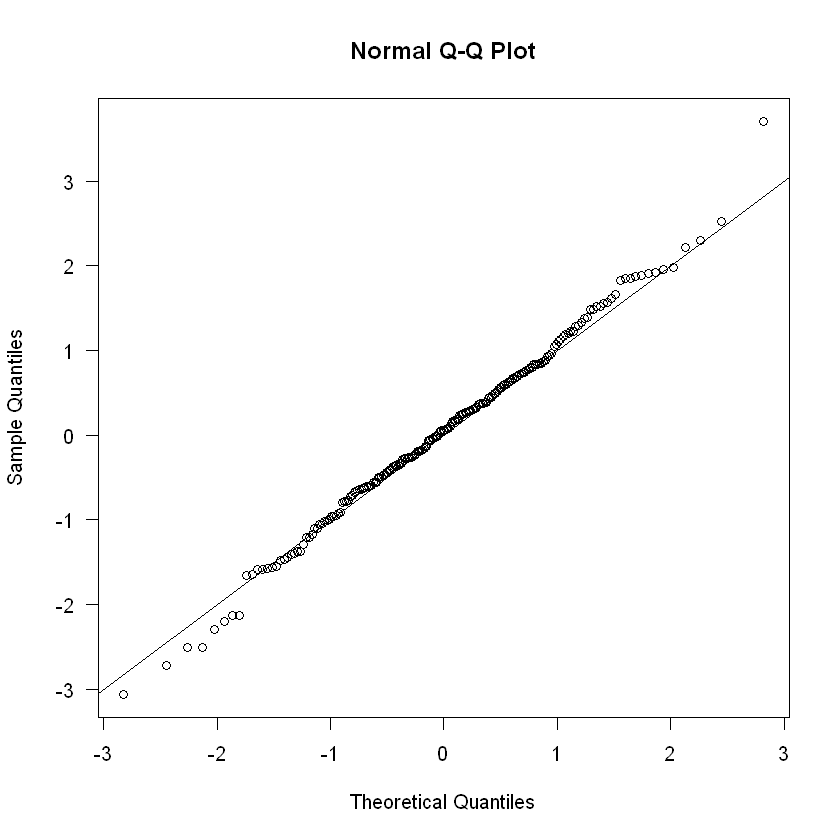
\includegraphics[width=\textwidth]{figures/minmax_mf_quantile_resid.png}
            \caption{Quantile residual của mô hình forward (dữ liệu được tiền xử lý minmax)}
        \end{subfigure}
        \hfill
        \begin{subfigure}[b]{0.4\textwidth}
            \centering
            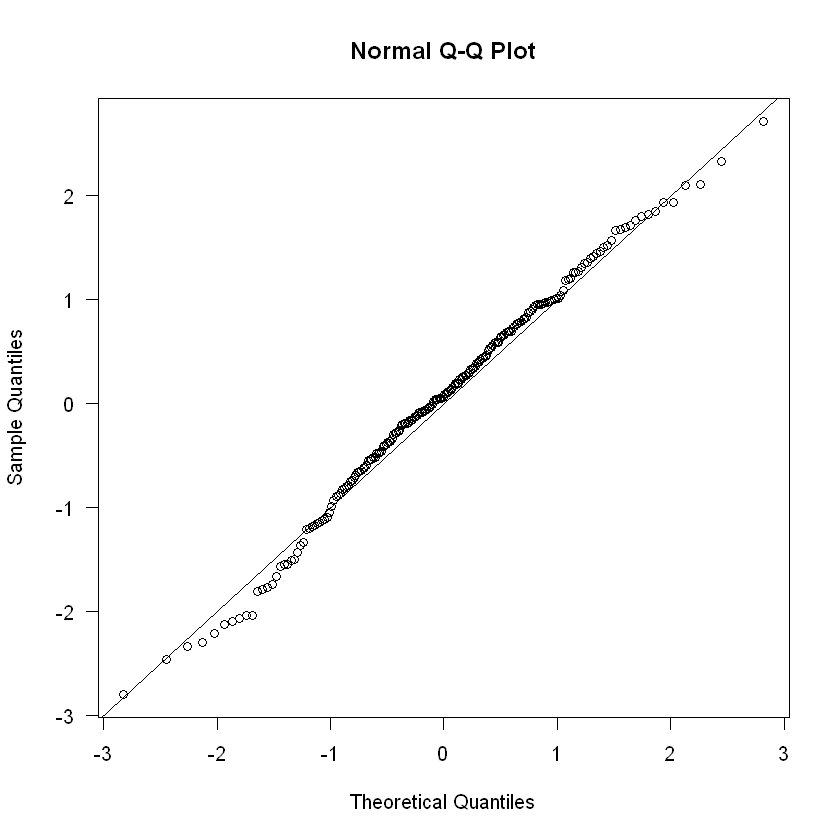
\includegraphics[width=\textwidth]{figures/standardize_mf_quantile_resid.png}
            \caption{Quantile residual của mô hình forward (dữ liệu được tiền xử lý standardize)}
        \end{subfigure}
        \label{fig:Quantile-resid-mf}
    \end{figure}

    \begin{figure}[h!]
        \centering
        \begin{subfigure}[b]{0.4\textwidth}
            \centering
            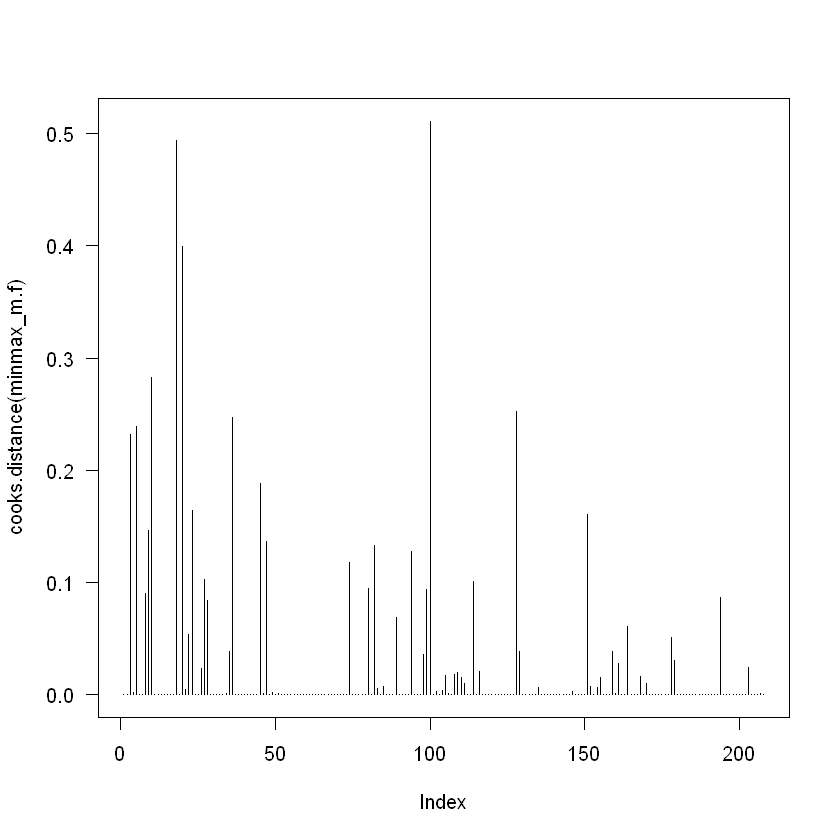
\includegraphics[width=\textwidth]{figures/minmax_mf_cooks.png}
            \caption{Cooks distance của mô hình forward (dữ liệu được tiền xử lý minmax)}
        \end{subfigure}
        \hfill
        \begin{subfigure}[b]{0.4\textwidth}
            \centering
            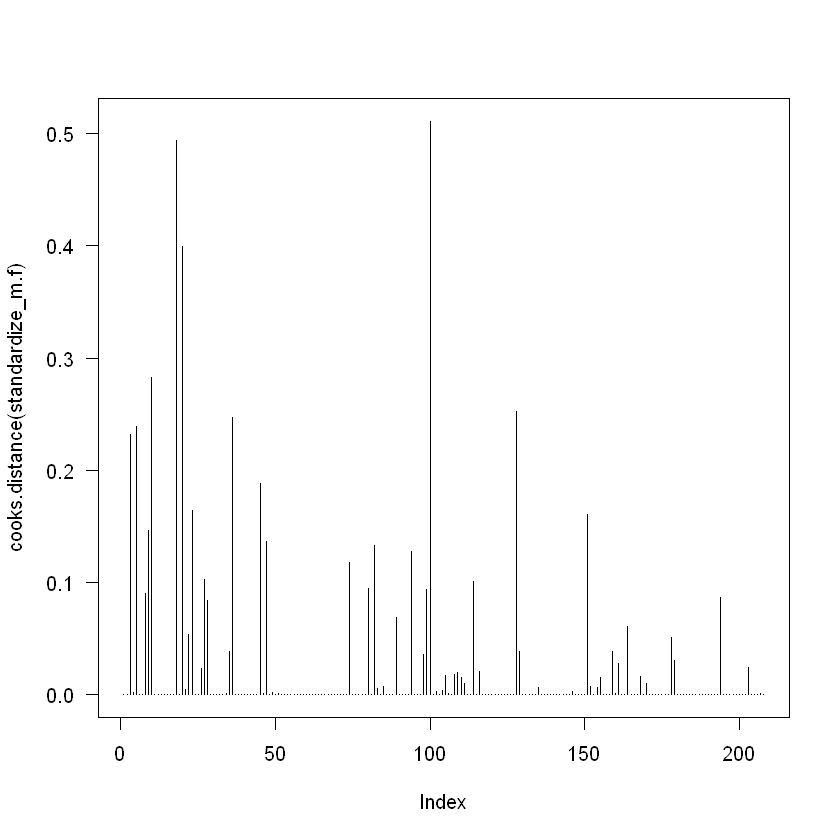
\includegraphics[width=\textwidth]{figures/standardize_mf_cooks.png}
            \caption{Cooks distance của mô hình forward (dữ liệu được tiền xử lý standardize)}
        \end{subfigure}
        \label{fig:Cooks-distance-mf}
    \end{figure}


    \begin{figure}[h!]
        \centering
        \begin{subfigure}[b]{0.4\textwidth}
            \centering
            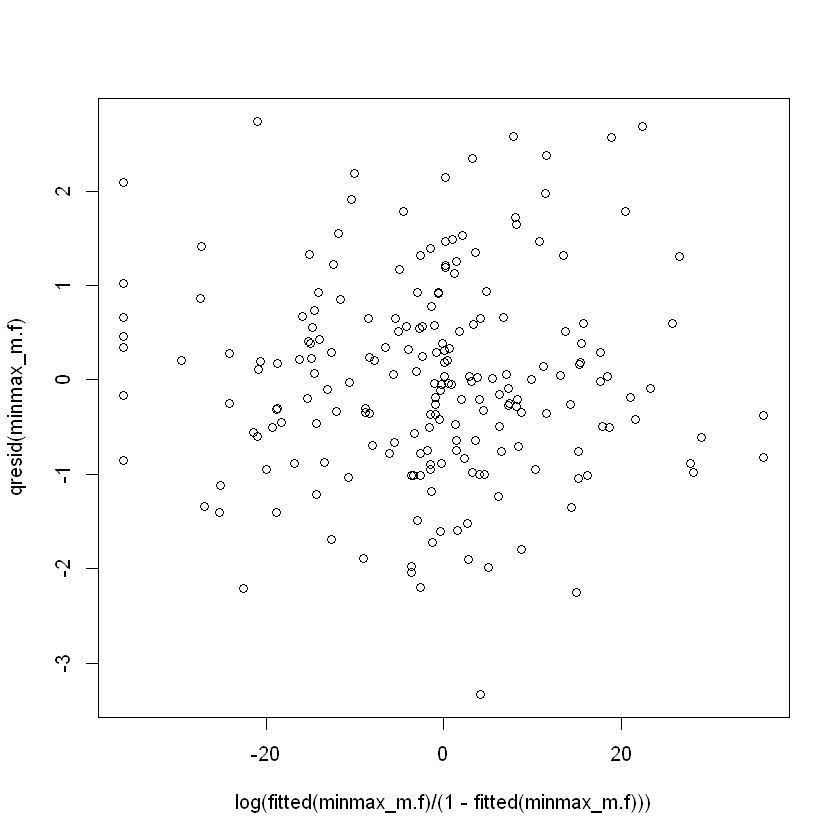
\includegraphics[width=\textwidth]{figures/minmax_mf_fitted.png}
            \caption{Quantile residual theo fitted value của mô hình forward (dữ liệu được tiền xử lý minmax)}
        \end{subfigure}
        \hfill
        \begin{subfigure}[b]{0.4\textwidth}
            \centering
            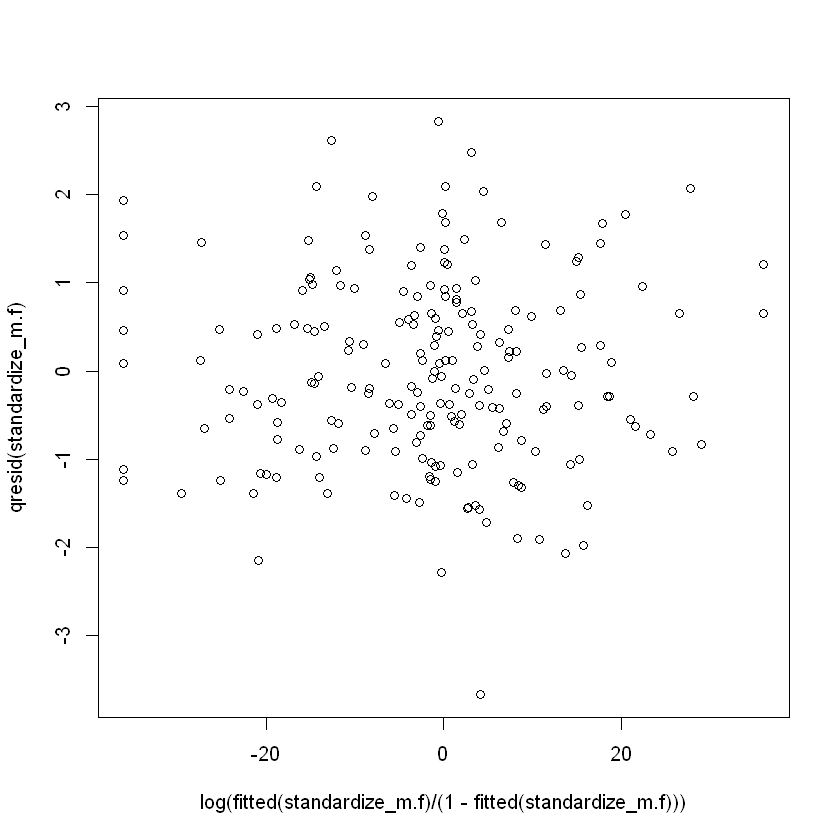
\includegraphics[width=\textwidth]{figures/standardize_mf_fitted.png}
            \caption{Quantile residual theo fitted value của mô hình forward (dữ liệu được tiền xử lý standardize)}
        \end{subfigure}
        \label{fig:Quantile-fitted-mf}
    \end{figure}

    Ta kiểm định các hệ số của mô hình forward sử dụng likelihood ratio test:

    \begin{verbatim}
anova(minmax_m.b, test="Chisq")
    \end{verbatim}

    \begin{verbatim}
Df	Deviance	Resid. Df	Resid. Dev	Pr(>Chi)
<int>	<dbl>	<int>	<dbl>	<dbl>
NULL	NA	NA	207	2.874062e+02	NA
V1	1	17.713882964	206	2.696923e+02	2.567460e-05
V3	1	0.605538874	205	2.690868e+02	4.364725e-01
V7	1	0.401073639	204	2.686857e+02	5.265353e-01
V9	1	16.415841846	203	2.522699e+02	5.085840e-05
V12	1	18.464018055	202	2.338059e+02	1.731425e-05
V13	1	0.040230414	201	2.337656e+02	8.410307e-01
V14	1	1.482925834	200	2.322827e+02	2.233173e-01
V16	1	2.775377941	199	2.295073e+02	9.572406e-02
V17	1	0.040139972	198	2.294672e+02	8.412072e-01
V18	1	2.554980373	197	2.269122e+02	1.099472e-01
V19	1	9.888496760	196	2.170237e+02	1.663152e-03
V20	1	0.100063203	195	2.169236e+02	7.517538e-01
V21	1	8.718785951	194	2.082049e+02	3.149477e-03
V22	1	4.578958193	193	2.036259e+02	3.236689e-02
V23	1	0.688625865	192	2.029373e+02	4.066322e-01
V24	1	0.007890769	191	2.029294e+02	9.292170e-01
V25	1	0.173935050	190	2.027554e+02	6.766380e-01
V27	1	1.067674920	189	2.016878e+02	3.014712e-01
V29	1	1.307537307	188	2.003802e+02	2.528410e-01
V30	1	0.037764676	187	2.003425e+02	8.459164e-01
V31	1	7.187290937	186	1.931552e+02	7.342175e-03
V32	1	4.891994149	185	1.882632e+02	2.698150e-02
V33	1	6.664572192	184	1.815986e+02	9.834826e-03
V34	1	2.380619623	183	1.792180e+02	1.228488e-01
V37	1	5.647405508	182	1.735706e+02	1.748122e-02
V39	1	3.342750615	181	1.702278e+02	6.750168e-02
V40	1	0.003614541	180	1.702242e+02	9.520592e-01
V41	1	8.616473888	179	1.616077e+02	3.331361e-03
V42	1	4.215551288	178	1.573922e+02	4.005505e-02
V43	1	2.942413740	177	1.544498e+02	8.628171e-02
V46	1	12.732911806	176	1.417169e+02	3.592767e-04
V48	1	18.532618731	175	1.231842e+02	1.670213e-05
V50	1	11.198645365	174	1.119856e+02	8.185707e-04
V51	1	13.815457905	173	9.817014e+01	2.016702e-04
V52	1	24.175881404	172	7.399426e+01	8.792654e-07
V57	1	0.196456219	171	7.379781e+01	6.575966e-01
V58	1	73.797803271	170	2.848136e-06	8.654286e-18
    \end{verbatim}

    \begin{verbatim}
anova(standardize_m.b, test="Chisq")
    \end{verbatim}

    \begin{verbatim}
Df	Deviance	Resid. Df	Resid. Dev	Pr(>Chi)
<int>	<dbl>	<int>	<dbl>	<dbl>
NULL	NA	NA	207	2.874062e+02	NA
V1	1	17.713882964	206	2.696923e+02	2.567460e-05
V3	1	0.605538874	205	2.690868e+02	4.364725e-01
V7	1	0.401073639	204	2.686857e+02	5.265353e-01
V9	1	16.415841846	203	2.522699e+02	5.085840e-05
V12	1	18.464018055	202	2.338059e+02	1.731425e-05
V13	1	0.040230414	201	2.337656e+02	8.410307e-01
V14	1	1.482925834	200	2.322827e+02	2.233173e-01
V16	1	2.775377941	199	2.295073e+02	9.572406e-02
V17	1	0.040139972	198	2.294672e+02	8.412072e-01
V18	1	2.554980373	197	2.269122e+02	1.099472e-01
V19	1	9.888496760	196	2.170237e+02	1.663152e-03
V20	1	0.100063203	195	2.169236e+02	7.517538e-01
V21	1	8.718785951	194	2.082049e+02	3.149477e-03
V22	1	4.578958193	193	2.036259e+02	3.236689e-02
V23	1	0.688625865	192	2.029373e+02	4.066322e-01
V24	1	0.007890769	191	2.029294e+02	9.292170e-01
V25	1	0.173935050	190	2.027554e+02	6.766380e-01
V27	1	1.067674920	189	2.016878e+02	3.014712e-01
V29	1	1.307537307	188	2.003802e+02	2.528410e-01
V30	1	0.037764676	187	2.003425e+02	8.459164e-01
V31	1	7.187290937	186	1.931552e+02	7.342175e-03
V32	1	4.891994149	185	1.882632e+02	2.698150e-02
V33	1	6.664572192	184	1.815986e+02	9.834826e-03
V34	1	2.380619623	183	1.792180e+02	1.228488e-01
V37	1	5.647405508	182	1.735706e+02	1.748122e-02
V39	1	3.342750615	181	1.702278e+02	6.750168e-02
V40	1	0.003614541	180	1.702242e+02	9.520592e-01
V41	1	8.616473888	179	1.616077e+02	3.331361e-03
V42	1	4.215551288	178	1.573922e+02	4.005505e-02
V43	1	2.942413740	177	1.544498e+02	8.628171e-02
V46	1	12.732911806	176	1.417169e+02	3.592767e-04
V48	1	18.532618731	175	1.231842e+02	1.670213e-05
V50	1	11.198645365	174	1.119856e+02	8.185707e-04
V51	1	13.815457905	173	9.817014e+01	2.016702e-04
V52	1	24.175881404	172	7.399426e+01	8.792654e-07
V57	1	0.196456219	171	7.379781e+01	6.575966e-01
V58	1	73.797803271	170	2.848136e-06	8.654286e-18
        
    \end{verbatim}

    \begin{figure}[h!]
        \centering
        \begin{subfigure}[b]{0.4\textwidth}
            \centering
            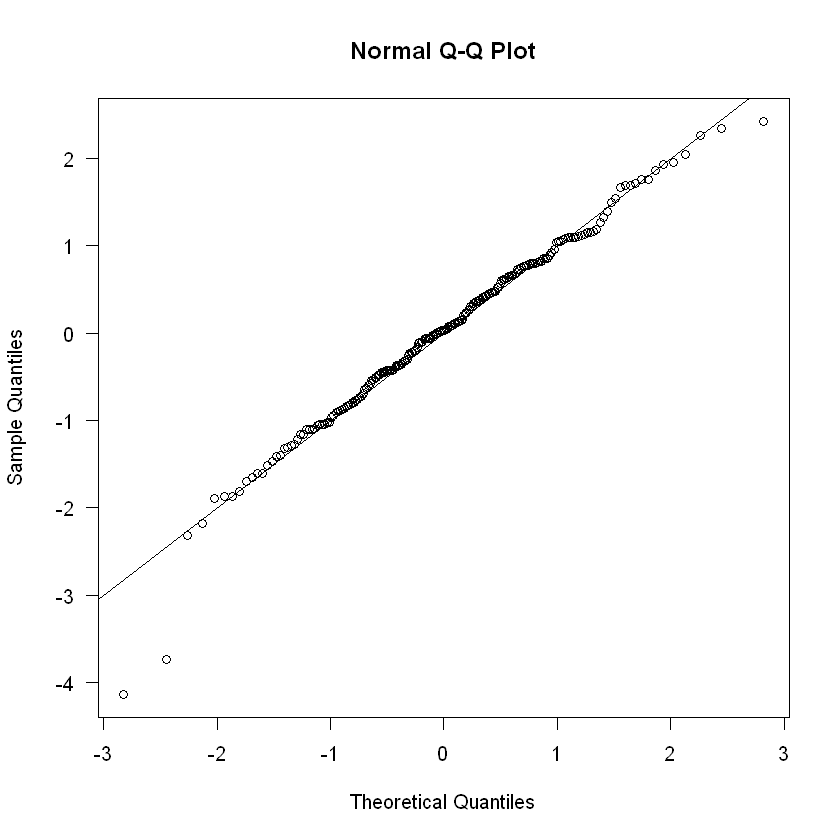
\includegraphics[width=\textwidth]{figures/minmax_mb_quantile_resid.png}
            \caption{Quantile residual của mô hình backward (dữ liệu được tiền xử lý minmax)}
        \end{subfigure}
        \hfill
        \begin{subfigure}[b]{0.4\textwidth}
            \centering
            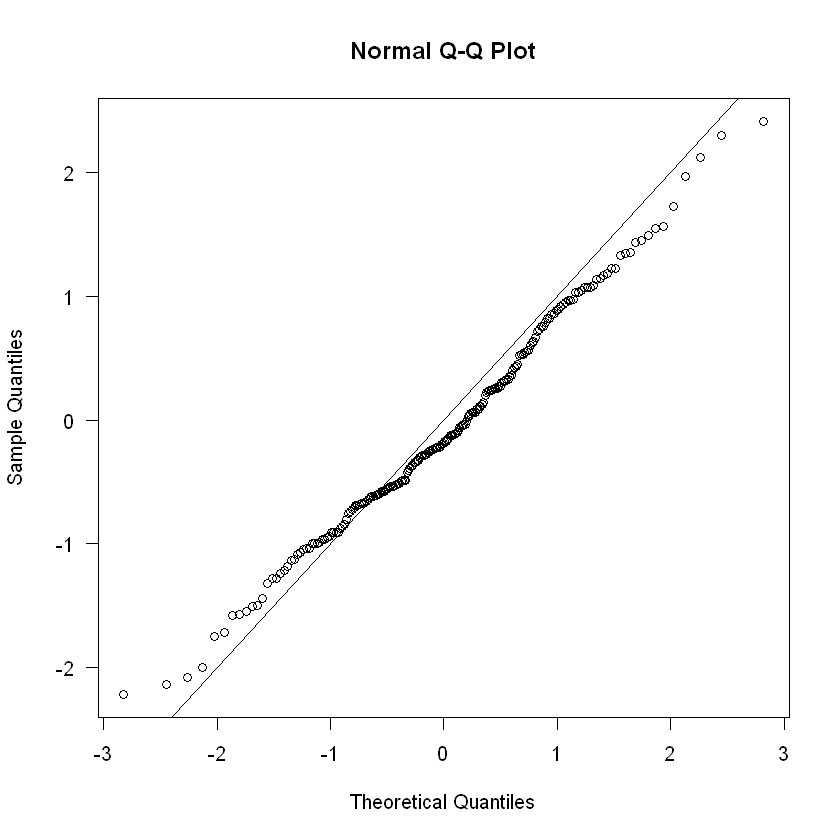
\includegraphics[width=\textwidth]{figures/standardize_mb_quantile_resid.png}
            \caption{Quantile residual của mô hình backward (dữ liệu được tiền xử lý standardize)}
        \end{subfigure}
        \label{fig:Quantile-resid-mb}
    \end{figure}


    \begin{figure}[h!]
        \centering
        \begin{subfigure}[b]{0.4\textwidth}
            \centering
            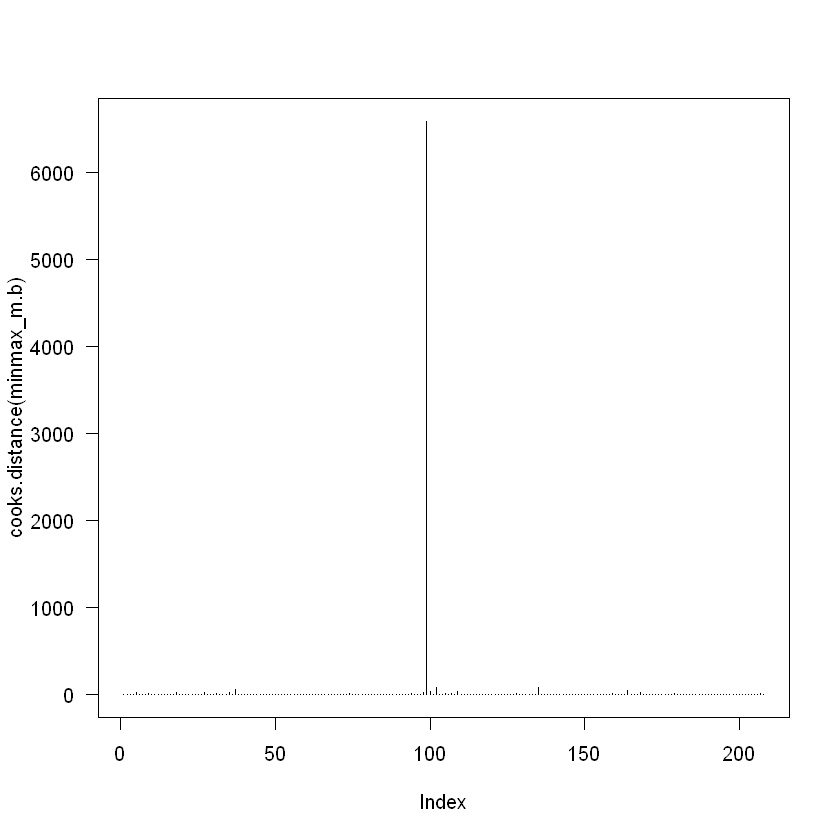
\includegraphics[width=\textwidth]{figures/minmax_mb_cooks.png}
            \caption{Cooks distance của mô hình backward (dữ liệu được tiền xử lý minmax)}
        \end{subfigure}
        \hfill
        \begin{subfigure}[b]{0.4\textwidth}
            \centering
            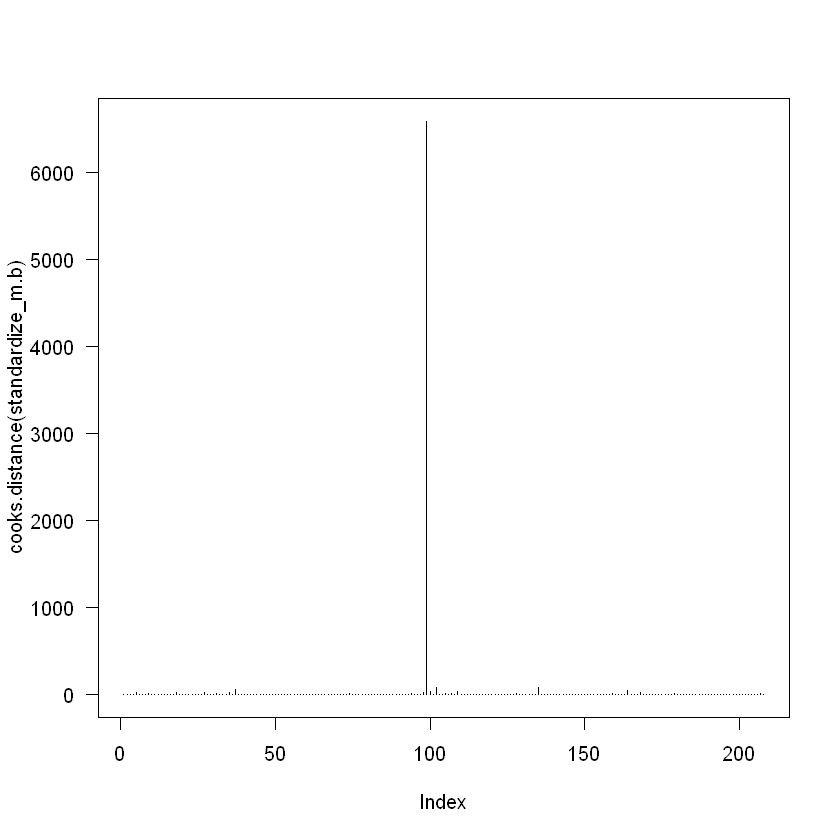
\includegraphics[width=\textwidth]{figures/standardize_mb_cooks.png}
            \caption{Cooks distance của mô hình backward (dữ liệu được tiền xử lý standardize)}
        \end{subfigure}
        \label{fig:Cooks-distance-mb}
    \end{figure}

    \begin{figure}[h!]
        \centering
        \begin{subfigure}[b]{0.4\textwidth}
            \centering
            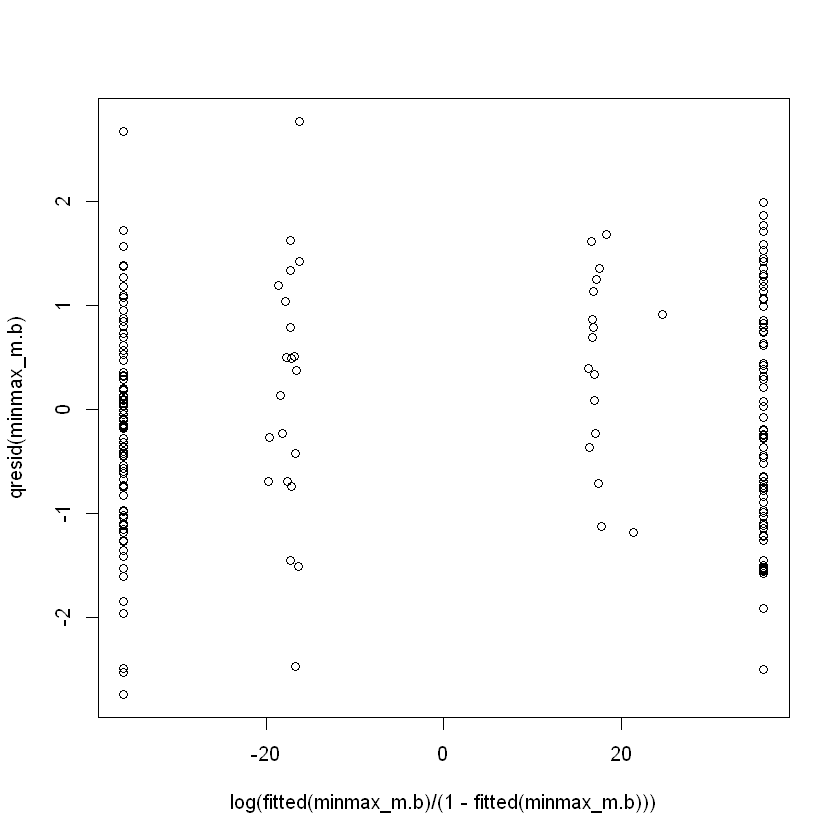
\includegraphics[width=\textwidth]{figures/minmax_mb_fitted.png}
            \caption{Quantile residual theo fitted value của mô hình backward (dữ liệu được tiền xử lý minmax)}
        \end{subfigure}
        \hfill
        \begin{subfigure}[b]{0.4\textwidth}
            \centering
            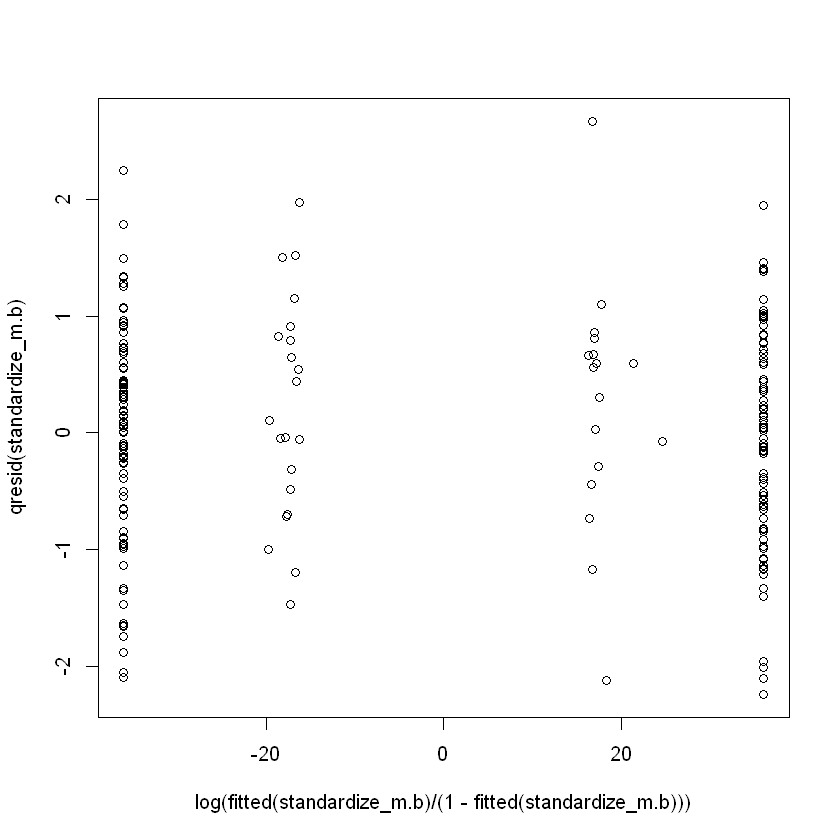
\includegraphics[width=\textwidth]{figures/standardize_mb_fitted.png}
            \caption{Quantile residual theo fitted value của mô hình backward (dữ liệu được tiền xử lý standardize)}
        \end{subfigure}
        \label{fig:Quantile-fitted-mb}
    \end{figure}

    Ta kiểm định các hệ số của mô hình forward sử dụng likelihood ratio test:

    \begin{verbatim}
anova(minmax_m.bo, test="Chisq")
    \end{verbatim}
    
    \begin{verbatim}
Df	Deviance	Resid. Df	Resid. Dev	Pr(>Chi)
<int>	<dbl>	<int>	<dbl>	<dbl>
NULL	NA	NA	207	287.4062	NA
V2	1	12.3993380	206	275.0069	4.294861e-04
V4	1	7.2353306	205	267.7715	7.148265e-03
V10	1	17.6355013	204	250.1360	2.675471e-05
V11	1	14.7399471	203	235.3961	1.234037e-04
V17	1	7.1135689	202	228.2825	7.650265e-03
V20	1	7.9403408	201	220.3422	4.834473e-03
V21	1	2.6332555	200	217.7089	1.046469e-01
V22	1	3.4019489	199	214.3070	6.511944e-02
V29	1	4.6766949	198	209.6303	3.057452e-02
V30	1	0.1571336	197	209.4731	6.918094e-01
V31	1	2.8813646	196	206.5918	8.961005e-02
V32	1	5.0170651	195	201.5747	2.509867e-02
V34	1	11.6135724	194	189.9611	6.547227e-04
V35	1	1.1156477	193	188.8455	2.908575e-01
V36	1	10.0702347	192	178.7753	1.506838e-03
V49	1	27.9711885	191	150.8041	1.231352e-07
V50	1	5.2407937	190	145.5633	2.206321e-02        
    \end{verbatim}

    \begin{verbatim}
anova(standardize_m.bo, test="Chisq")
    \end{verbatim}

    \begin{verbatim}
Df	Deviance	Resid. Df	Resid. Dev	Pr(>Chi)
<int>	<dbl>	<int>	<dbl>	<dbl>
NULL	NA	NA	207	287.4062	NA
V2	1	12.3993380	206	275.0069	4.294861e-04
V4	1	7.2353306	205	267.7715	7.148265e-03
V10	1	17.6355013	204	250.1360	2.675471e-05
V11	1	14.7399471	203	235.3961	1.234037e-04
V17	1	7.1135689	202	228.2825	7.650265e-03
V20	1	7.9403408	201	220.3422	4.834473e-03
V21	1	2.6332555	200	217.7089	1.046469e-01
V22	1	3.4019489	199	214.3070	6.511944e-02
V29	1	4.6766949	198	209.6303	3.057452e-02
V30	1	0.1571336	197	209.4731	6.918094e-01
V31	1	2.8813646	196	206.5918	8.961005e-02
V32	1	5.0170651	195	201.5747	2.509867e-02
V34	1	11.6135724	194	189.9611	6.547227e-04
V35	1	1.1156477	193	188.8455	2.908575e-01
V36	1	10.0702347	192	178.7753	1.506838e-03
V49	1	27.9711885	191	150.8041	1.231352e-07
V50	1	5.2407937	190	145.5633	2.206321e-02
    \end{verbatim}

    \begin{figure}[h!]
        \centering
        \begin{subfigure}[b]{0.4\textwidth}
            \centering
            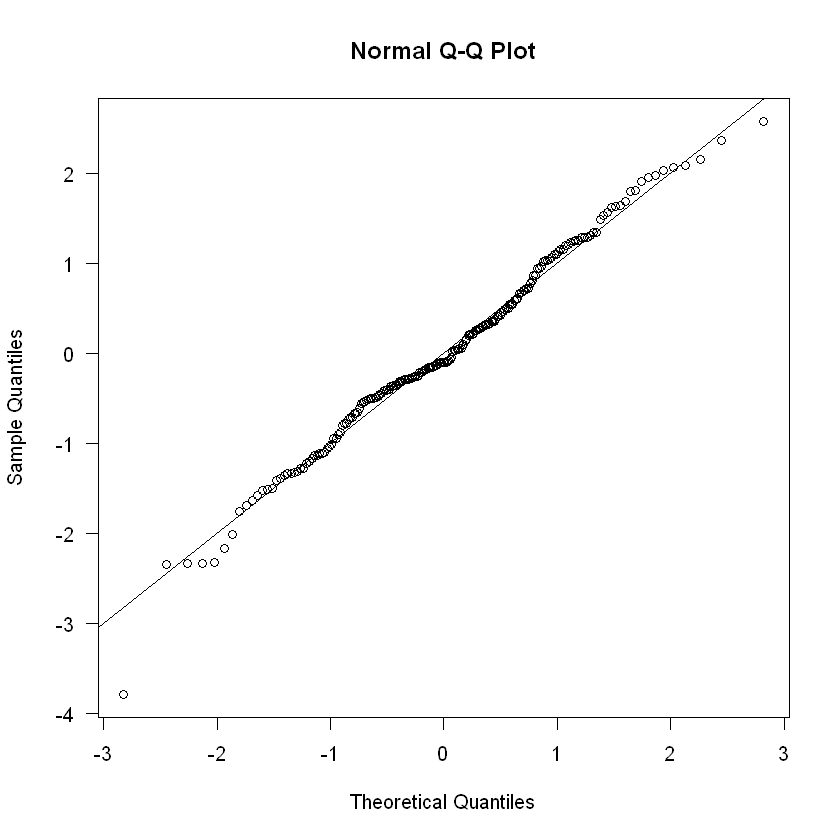
\includegraphics[width=\textwidth]{figures/minmax_mbo_quantile_resid.png}
            \caption{Quantile residual của mô hình forward-backward (dữ liệu được tiền xử lý minmax)}
        \end{subfigure}
        \hfill
        \begin{subfigure}[b]{0.4\textwidth}
            \centering
            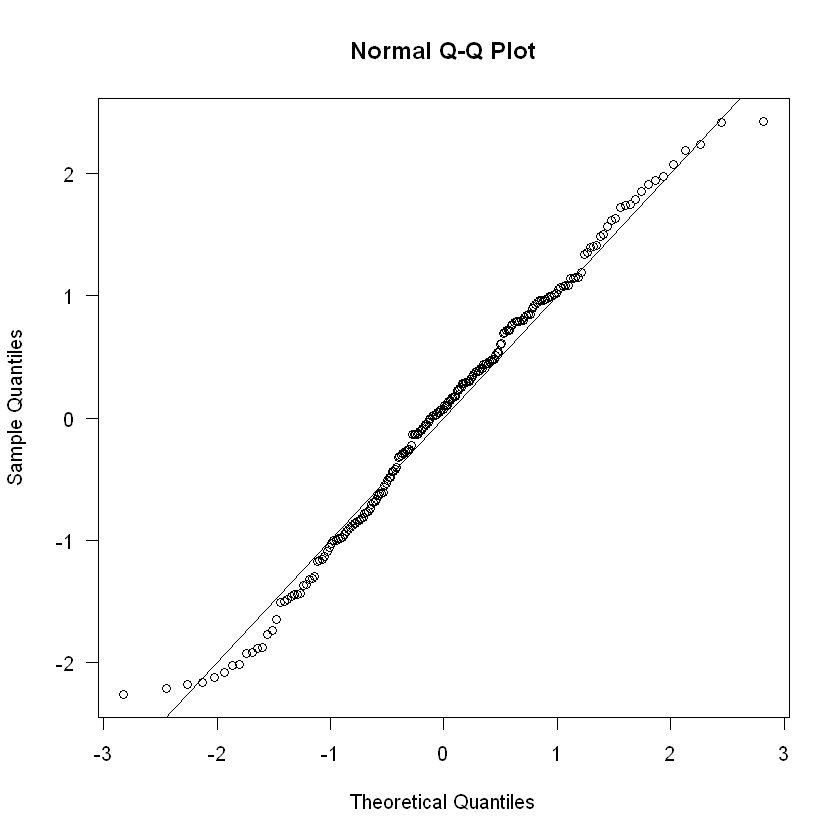
\includegraphics[width=\textwidth]{figures/standardize_mbo_quantile_resid.png}
            \caption{Quantile residual của mô hình forward-backward (dữ liệu được tiền xử lý standardize)}
        \end{subfigure}
        \label{fig:Quantile-resid-mbo}
    \end{figure}

    \begin{figure}[h!]
        \centering
        \begin{subfigure}[b]{0.4\textwidth}
            \centering
            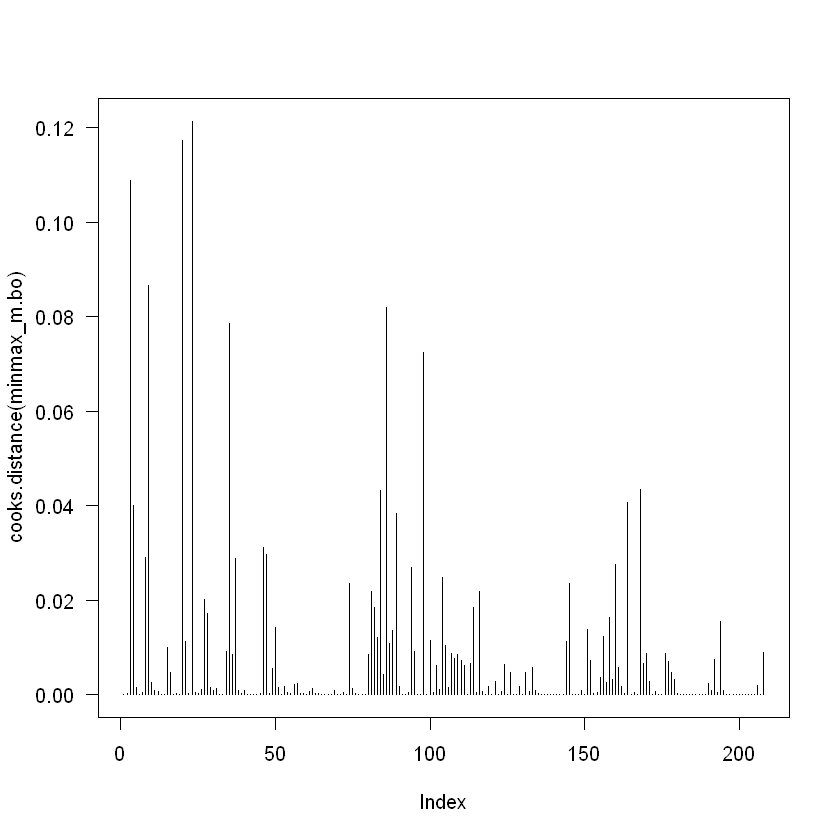
\includegraphics[width=\textwidth]{figures/minmax_mbo_cooks.png}
            \caption{Cooks distance của mô hình forward-backward (dữ liệu được tiền xử lý minmax)}
        \end{subfigure}
        \hfill
        \begin{subfigure}[b]{0.4\textwidth}
            \centering
            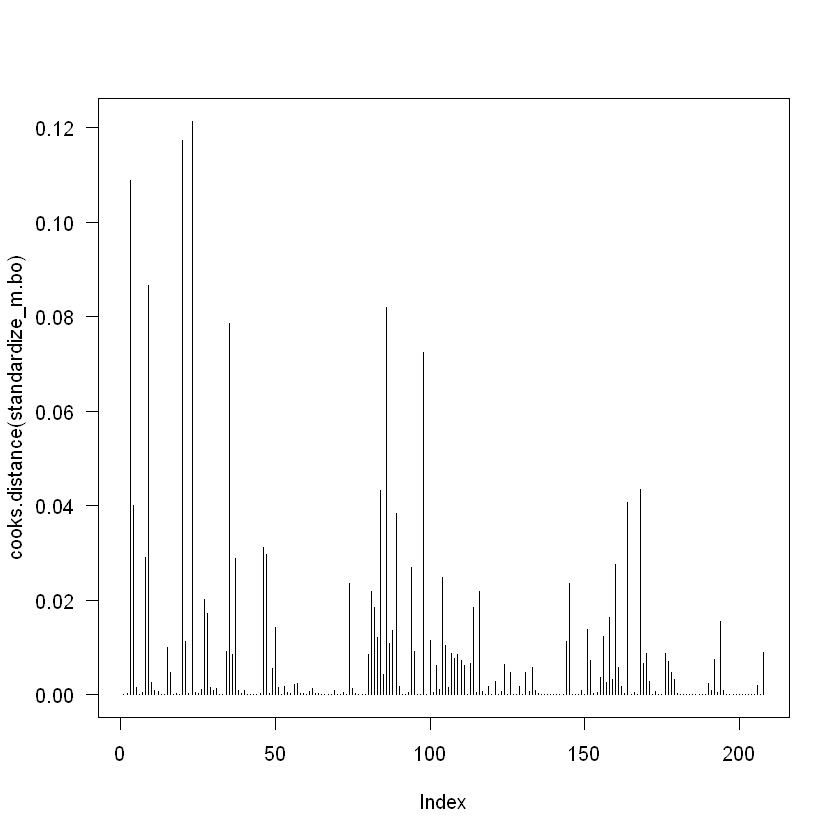
\includegraphics[width=\textwidth]{figures/standardize_mbo_cooks.png}
            \caption{Cooks distance của mô hình forward-backward (dữ liệu được tiền xử lý standardize)}
        \end{subfigure}
        \label{fig:Cooks-distance-mbo}
    \end{figure}

    \begin{figure}[h!]
        \centering
        \begin{subfigure}[b]{0.4\textwidth}
            \centering
            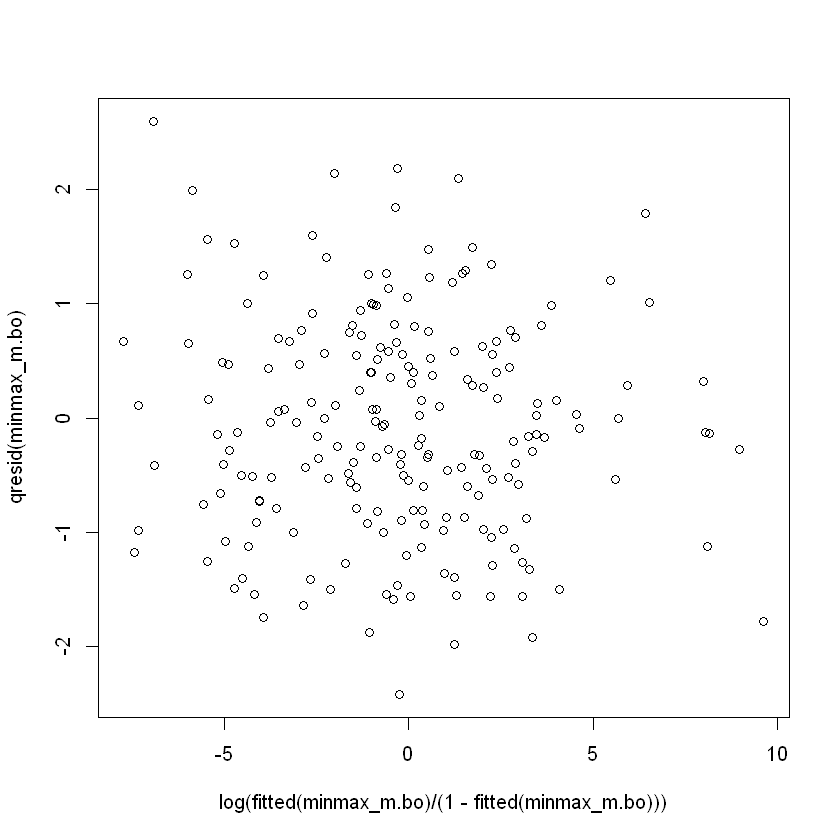
\includegraphics[width=\textwidth]{figures/minmax_mbo_fitted.png}
            \caption{Quantile residual theo fitted value của mô hình forward-backward (dữ liệu được tiền xử lý minmax)}
        \end{subfigure}
        \hfill
        \begin{subfigure}[b]{0.4\textwidth}
            \centering
            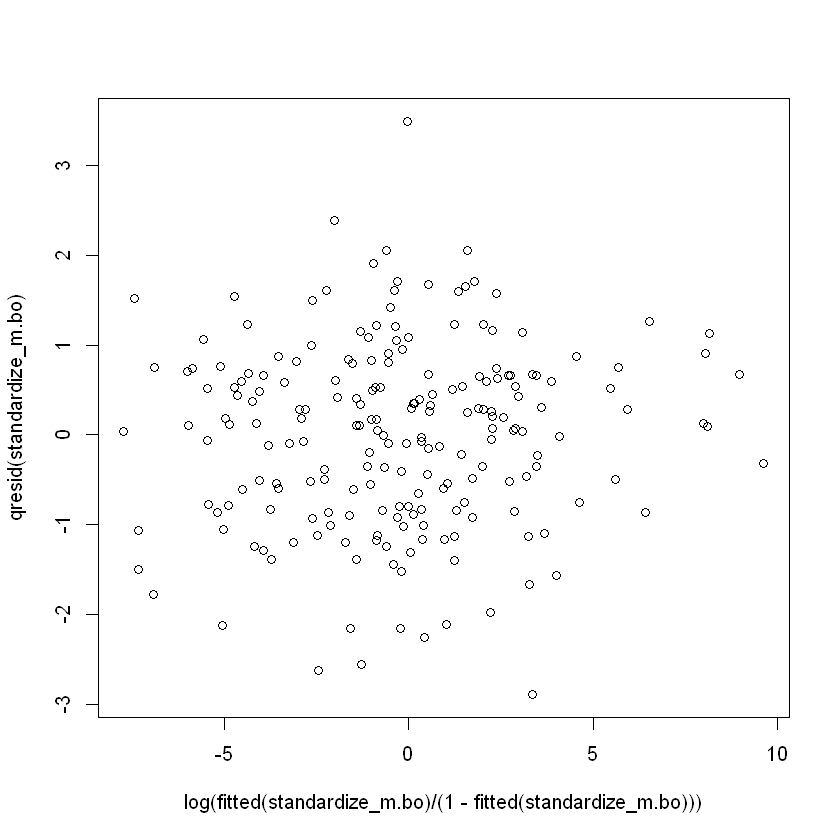
\includegraphics[width=\textwidth]{figures/standardize_mbo_fitted.png}
            \caption{Quantile residual theo fitted value của mô hình forward-backward (dữ liệu được tiền xử lý standardize)}
        \end{subfigure}
        \label{fig:Quantile-fitted-mbo}
    \end{figure}

    Tổng hợp lại sử dụng 5 mô hình:

    \begin{itemize}
        \item Mô hình gồm tất cả các biến (ký hiệu là full)
        \item Mô hình forward được chọn ở bài tập trước (ký hiệu là m.f)
        \item Mô hình backward được chọn ở bài tập trước (ký hiệu là m.b)
        \item Mô hình forward-backward được chọn ở bài tập trước (ký hiệu là m.bo)
        \item Mô hình các biến được trích xuất từ thuật toán PCA giữ lại 95 \% thông tin (ký hiệu là pca\_x với x là thuật toán PCA giữ lại x \% thông tin)
    \end{itemize}

    Để chọn ra mô hình tốt nhất, mỗi mô hình đi kèm với cách chỉnh định sẽ được tối ưu hóa các siêu tham số gồm:

    \begin{itemize}
        \item Phương pháp tiền xử lý: min-max scaling, standardize.
        \item Tốc độ học được biến đổi trong quá trình huấn luyện theo các cách: fixed, cyclic, inverse\_decay, exponential\_decay, factor\_decay, squareroot, cosine.
        \item Các tốc độ học khác nhau: 1e-4, 1e-3, 1e-2, 1e-1, 1, 2, 5, 10
        \item Các thuật toán tối ưu hóa, 12 thuật toán tối ưu hóa được sử dụng gồm:
        \begin{itemize}
            \item Gradient Descent
            \item Adam
            \item Avagrad
            \item RAdam
            \item Momentum
            \item Adagrad
            \item RMSProp
            \item Adadelta
            \item Adamax
            \item Nadam
            \item AMSGrad
            \item AdaBelief
        \end{itemize}

        Sơ đồ mã giả của các thuật toán tối ưu hóa được trình bày ở phụ lục \ref{Optimization-Algorithms} và chi tiết các phương pháp điều chỉnh tốc độ học được trình bày ở phục lục \ref{LRScheduler}
    \end{itemize}

    Các siêu tham số trên sẽ được huấn luyện sử dụng code python và numpy không sử dụng thư viện khác.
    Việc sử dụng code python và numpy để có thể thử với các thuật toán tối ưu hóa khác mà thư viện sklearn không có.
    Hệ số $\lambda$ trong quá trình huấn luyện các mô hình được tự cài đặt bằng python và numpy được cố định là 1e-3 (do hạn chế về mặt thời gian).
    Kết quả của quá trình tối ưu hóa siêu tham số cho các mô hình được cài đặt bằng python và numpy được trình bày ở bảng \ref{tab:custom-hyperparameter-result} với cột bên trái ngoài cùng là loại mô hình (được hình thành từ các biến giải thích sử dụng và phương pháp chỉnh định) các cột bên phải là tổ hợp các siêu tham số tối ưu tương ứng.

    Ngoài ra ta vẫn huấn luyện một tập các mô hình được huấn luyện sử dụng thư viện sklearn.
    Vì vấn đề thời gian đối với các mô hình được huấn luyện trên sklearn chỉ gồm 3 mô hình:
    \begin{itemize}
        \item Mô hình gồm tất cả các biến
        \item Mô hình forward-backward
        \item Mô hình các biến được trích xuất từ thuật toán PCA giữ lại 95 \% thông tin
    \end{itemize}
    Siêu tham số của các mô hình được huấn luyện sử dụng sklearn bao gồm:

    \begin{itemize}
        \item Phương pháp tiền xử lý: min-max scaling, standardize.
        \item Các hệ số $C$ là nghịch đảo của $\lambda$
        \item Các thuật toán tối ưu hóa, 6 thuật toán tối ưu hóa được sử dụng gồm:
        \begin{itemize}
            \item lbfgs
            \item liblinear
            \item newton-cg 
            \item newton-cholesky
            \item sag 
            \item saga
        \end{itemize}
    \end{itemize}

    Phương pháp chỉnh định "l1" được gọi là Lasso, phương pháp chỉnh định "l2" được gọi là Ridge, không chỉnh định ta gọi là Naive
    Mỗi một cặp thông tin gồm phương pháp chỉnh định ("l1", "l2", không chỉnh định) và mô hình sẽ được chọn ra bộ siêu tham số tốt nhất từ các siêu tham số được đề cập ở trên bằng độ đo AUC-ROC trên tập test.
    Ta sẽ cố định tập test ngay từ đầu.
    Như vậy ta sẽ có 5 (mô hình) $\times$ 3 ("l1"-lasso, "l2"-ridge, không chỉnh định) = 15 mô hình ứng viên được cài đặt bằng ngôn ngữ python và numpy được chọn từ quá trình tối ưu hóa siêu tham số và 9 mô hình ứng viên được huấn luyện bằng thư viện sklearn.
    Như vậy ta có 24 mô hình ứng viên.

    Từ các mô hình ứng viên, để chọn ra mô hình tốt nhất từ nhiều yếu tố như $AUC-ROC, AIC, BIC$ cũng như từ trung bình hình học G-Means giữa độ nhạy (Sensitivity) và độ đặc hiệu (Specificity) ứng với ngưỡng xác suất $p^*$ ($p^*$ làm cho G-Means cực đại) được chọn.

    \begin{table}[h!]
        \centering
        \begin{tabular}{|c | c | c | c | c |}
            \hline
            Mô hình & Phương pháp chuẩn hóa & Thuật toán tối ưu & Scheduler & Init learning rate \\
            \hline
            \hline
            full - Naive & standardize & RMSProp & inverse decay & 5 \\
            \hline
            m.bo - Naive & standardize & AdaBelief & fixed & 5 \\
            \hline
            m.f - Naive & standardize & RMSProp & squareroot &5 \\
            \hline
            m.b - Naive & standardize & RMSProp & cosine & 1 \\
            \hline
            pca\_95 - Naive & standardize & Gradient\_Descent & inverse\_decay & 10 \\
            \hline
            full - Lasso & minmax & Avagrad & squareroot & 10 \\
            \hline
            m.bo - Lasso & standardize & Adam & exponential\_decay & 10 \\
            \hline
            m.f - Lasso & standardize & RMSProp & fixed &2 \\
            \hline
            m.b - Lasso & standardize & AMSGrad & cyclic & 5 \\
            \hline
            pca\_95 - Lasso & standardize & Gradient\_Descent & cosine & 0.01 \\
            \hline
            full - Ridge & standardize & RAdam & fixed & 10 \\
            \hline
            m.bo - Ridge & standardize & Adam & fixed & 5 \\
            \hline
            m.f - Ridge & standardize & RAdam & fixed & 10 \\
            \hline
            m.b - Ridge & standardize & RAdam & fixed & 10 \\
            \hline
            pca\_95 - Ridge & standardize & RAdam & fixed & 10 \\
            \hline
        \end{tabular}
        \caption{Các siêu tham số tốt nhất với từng mô hình (mỗi mô hình được xác định bằng các biến \\ giải thích và phương pháp chỉnh định (naive, ridge, lasso))}
        \label{tab:custom-hyperparameter-result}
    \end{table}


    \begin{table}[h!]
        \centering
        \begin{tabular}{|c | c | c | c | c |}
            \hline
            Mô hình & Random\_state & Phương pháp chuẩn hóa & Thuật toán tối ưu & C \\
            \hline
            \hline
            Sklearn full - Naive & 379 & minmax & sag & 0.0001 \\
            \hline
            Sklearn m.bo - Naive & 953 & standardize & sag & 0.0001 \\
            \hline
            Sklearn pca\_95 - Naive & 431 & minmax & sag & 0.0001 \\
            \hline
            Sklearn full - Lasso & 587 & standardize & saga & 1000 \\
            \hline
            Sklearn m.bo - Lasso & 0 & standardize & liblinear & 10 \\
            \hline
            Sklearn pca\_95 - Lasso & 2 & minmax & saga & 0.1 \\
            \hline
            Sklearn full - Ridge & 0 & minmax & lbfgs & 10 \\
            \hline
            Sklearn m.bo - Ridge & 85 & standardize & sag & 100 \\
            \hline
            Sklearn pca\_95 - Ridge & 0 & minmax & lbfgs & 10 \\
            \hline
        \end{tabular}
        \caption{Các siêu tham số tốt nhất với từng mô hình được huấn luyện sử dụng thư viện sklearn (mỗi mô hình được xác định bằng các biến giải thích và phương pháp chỉnh định (naive, ridge, lasso))}
        \label{tab:sklearn-hyperparameter-result}
    \end{table}

    Random\_state được chính là seed để khởi tạo các tham số của mô hình.
    Còn tập dữ liệu được chia tập train và tập test một cách cố định từ ban đầu (sử dụng random\_state 42)

    Kết quả của quá trình tối ưu hóa siêu tham số cho các mô hình được cài đặt bằng python và numpy được trình bày ở bảng \ref{tab:sklearn-hyperparameter-result}


    Để chọn ra ngưỡng xác suất $p^*$ tốt nhất với từng mô hình ta tìm ngưỡng xác suất sao cho cực đại hóa trung bình hình học giữa độ nhạy (Sensitivity) và độ đặc hiệu (Specificity).
    Ta có công thức tính các đại lượng trên:

    \begin{equation*}
        \begin{aligned}
            \mathrm{TPR} = \mathrm{Precision} = \mathrm{Sensitivity} &= \dfrac{\mathrm{TP}}{\mathrm{TP} + \mathrm{FN}} \\
            \mathrm{FPR} &= \dfrac{\mathrm{FP}}{\mathrm{FP} + \mathrm{TN}} \\
            \mathrm{Specificity} = 1 - \mathrm{FPR} &= \dfrac{\mathrm{TN}}{\mathrm{FP} + \mathrm{TN}}
        \end{aligned}
    \end{equation*}

    Trung bình hình học giữa giữa độ nhạy (Sensitivity) và độ đặc hiệu (Specificity) là:
    \begin{equation*}
        \mathrm{G-Means} = \sqrt{\mathrm{Sensitivity} \times \mathrm{Specificity}} = \sqrt{\dfrac{\mathrm{TP}}{\mathrm{TP} + \mathrm{FN}} \times \dfrac{\mathrm{TN}}{\mathrm{FP} + \mathrm{TN}}}
    \end{equation*}

    Như ta đã biết đường cong ROC được xây dựng bằng cách chọn các ngưỡng xác suất $p$ để một mẫu được phân loại thành nhãn 1 hay nhãn 0 (mẫu được xem là nhãn 1 nếukết quả đầu ra lớn hơn 1 và ngược lại được xem là nhãn 0).
    Như vậy với mỗi ngưỡng xác suất sẽ có một bảng ma trận nhầm lẫn khác nhau (TP, TN, FP, FN thay đổi dựa theo ngưỡng xác suất) hay sẽ có các giá trị độ nhạy (Sensitivity) và độ đặc hiệu (Specificity) khác nhau từ đó dẫn đến trung bình hình học G-Means giữa hai đại lượng này cũng thay đổi.
    Ta chọn $p^*$ sao cho làm cực đại hóa giá trị G-Means:

    \begin{equation*}
        p^* = \underset{p}{\mathrm{argmax}} \mathrm{G-Means} = \underset{p}{\mathrm{argmax}} \sqrt{\mathrm{Sensitivity} \times \mathrm{Specificity}} = \underset{p}{\mathrm{argmax}} \sqrt{\dfrac{\mathrm{TP}}{\mathrm{TP} + \mathrm{FN}} \times \dfrac{\mathrm{TN}}{\mathrm{FP} + \mathrm{TN}}}
    \end{equation*}

    Để tính giá trị $p^*$ ta sử dụng đoạn code sau:

    \begin{python}
y_pred = model.predict(x=test_x, return_prob=True)
fpr, tpr, thresholds = roc_curve(y_true=test_y, y_score=y_pred)
area_roc = auc(fpr, tpr)
gmeans = compute_gmeans(tpr=tpr, fpr=fpr)
        
idx = np.argmax(gmeans)
prob_star = thresholds[idx]
gmean_star = gmeans[idx]
    \end{python}

    \begin{figure}[h!]
        \centering
        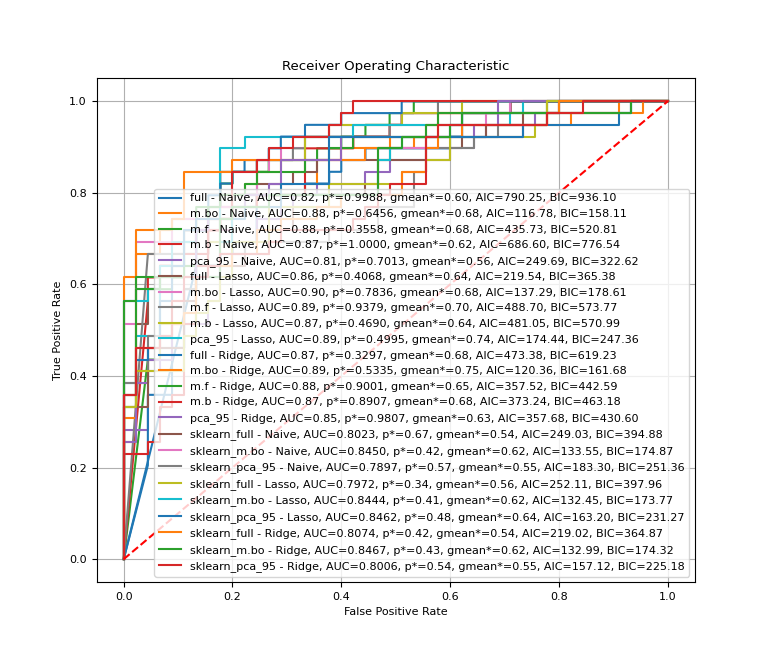
\includegraphics[width=1.0\textwidth]{figures/roc_curve_summary.png}
        \caption{Tổng hợp kết quả các mô hình}
        \label{fig:roc_curve_summary}
    \end{figure}

    \begin{figure}[h!]
        \centering
        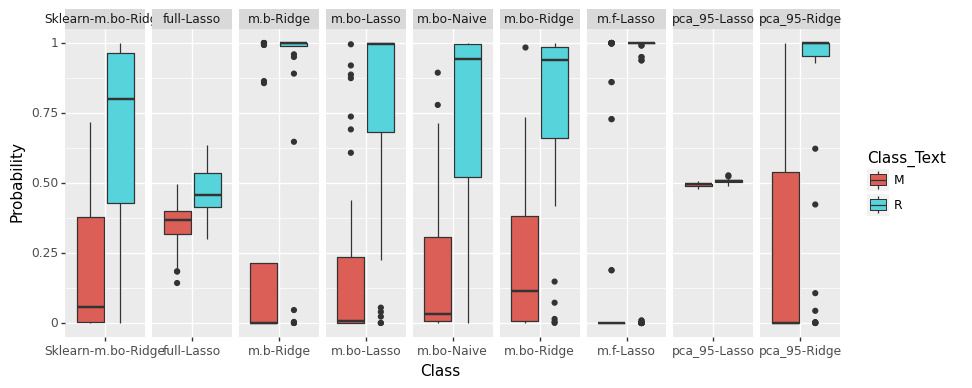
\includegraphics[width=1.0\textwidth]{figures/prob_box_plot.png}
        \caption{So sánh kết quả đầu ra của một số mô hình dùng box plot}
        \label{fig:prob_box_plot}
    \end{figure}

    \begin{figure}[h!]
        \centering
        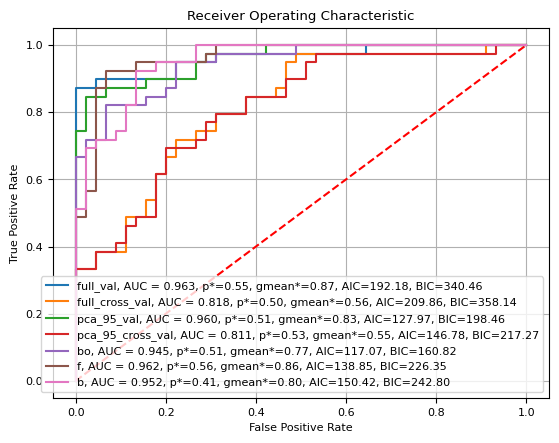
\includegraphics[width=1.0\textwidth]{figures/ROC_Curve_AIC_BIC_Excercise_2_1.png}
        \caption{ So sánh đường cong ROC, $p^*$, G-Means tương ứng với $p^*$, chỉ số AIC, BIC của các mô hình được tối ưu hóa tham số ở bài tập 2 theo cách 1}
        \label{fig:ROC_Curve_AIC_BIC_Excercise_2_1}
    \end{figure}

    \begin{figure}[h!]
        \centering
        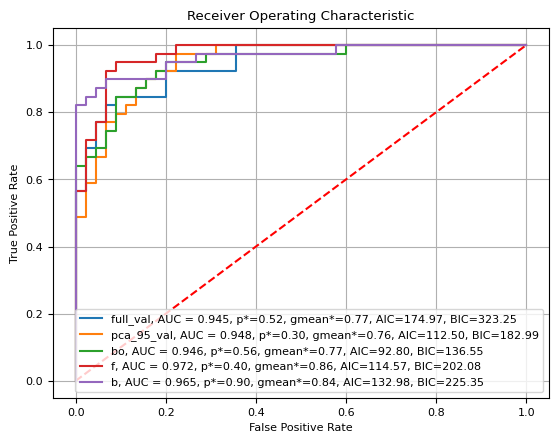
\includegraphics[width=1.0\textwidth]{figures/ROC_Curve_AIC_BIC_Excercise_2_2.png}
        \caption{ So sánh đường cong ROC, $p^*$, G-Means tương ứng với $p^*$, chỉ số AIC, BIC của các mô hình được tối ưu hóa tham số ở bài tập 2 theo cách 2}
        \label{fig:ROC_Curve_AIC_BIC_Excercise_2_2}
    \end{figure}
\end{loigiai}

\newpage
\printbibliography[title={TÀI LIỆU THAM KHẢO}]

\newpage
\appendix

\section{Các thuật toán tối ưu hóa} \label{Optimization-Algorithms}


\begin{algorithm}[h!]
    \DontPrintSemicolon
    \KwIn{độ dài bước $\lbrace \alpha_t \rbrace_{t=1}^{T}$, $w_0$ khởi tạo, hàm mục tiêu $\ell(w)$}
    \KwOut{$w$ đã được học}

    \For{$t \gets 1$ \KwSty{to} $T$} {
        $g_t \gets \nabla \ell(w_{t-1})$\;
        $w_t \gets w_{t-1} - \alpha_t g_t$
    }
    \Return{$w_T$}\;
    \caption{Thuật toán Gradient Descent}
\end{algorithm}


\begin{algorithm}[h!]
    \DontPrintSemicolon
    \KwIn{độ dài bước $\lbrace \alpha_t \rbrace_{t=1}^{T}$, hệ số $\beta_1$, $w_0$ khởi tạo, hàm mục tiêu $\ell(w)$}
    \KwOut{$w$ đã được học}
    $m_0 \gets 0$\;
    \For{$t \gets 1$ \KwSty{to} $T$} {
        $g_t \gets \nabla \ell(w_{t-1})$\;
        $m_t \gets \beta_1 m_{t-1} + (1-\beta_1) g_t$\;
        $w_t \gets w_{t-1} - \alpha_t m_t$\;
    }
    \Return{$w_T$}\;
    \caption{Thuật toán Momentum}
\end{algorithm}


\begin{algorithm}[h!]
    \KwIn{độ dài bước $\lbrace \alpha_t \rbrace_{t=1}^{T}$, $w_0$ khởi tạo, hàm mục tiêu $\ell(w)$}
    \KwOut{$w$ đã được học}

    $v_0 \gets 0$\;
    \For{$t \gets 1$ \KwSty{to} $T$} {
        $g_t \gets \nabla \ell(w_{t-1})$\;
        $v_t \gets v_{t-1} + g_t^2$\;
        $w_t \gets w_{t-1} - \alpha_t \dfrac{g_t}{\sqrt{v_t} + \epsilon}$\;
    }

    \Return{$w_T$}\;
    \caption{Thuật toán Adagrad}
\end{algorithm}

\begin{algorithm}[h!]
    \DontPrintSemicolon
    \KwIn{độ dài bước $\lbrace \alpha_t \rbrace_{t=1}^{T}$, hệ số $\beta$, $w_0$ khởi tạo, hàm mục tiêu $\ell(w)$}
    \KwOut{$w$ đã được học}

    $v_0 \gets 0$\;
    $d_0 \gets 0$\;

    \For{$t \gets 1$ \KwSty{to} $T$} {
        $g_t \gets \nabla \ell (w_{t-1})$\;
        $v_t \gets \beta v_{t-1} + (1-\beta) g_t^2$\;
        $\Delta w \gets -\alpha_t \dfrac{\sqrt{d_{t-1} + \epsilon}g_t}{\sqrt{v_t + \epsilon}}$\;
        $w_t \gets w_{t-1} + \delta w$\;
        $d_t \gets \beta d_{t-1} + (1-\beta) \delta w^2$\;
    }

    \Return{$w_T$}\;
    \caption{Thuật toán Adadelta}
\end{algorithm}


\begin{algorithm}[h!]
    \DontPrintSemicolon
    \KwIn{độ dài bước $\lbrace \alpha_t \rbrace_{t=1}^{T}$, hệ số $\beta$, $w_0$ khởi tạo, hàm mục tiêu $\ell(w)$}
    \KwOut{$w$ đã được học}

    $v_0 \gets 0$\;
    \For{$t \gets 1$ \KwSty{to} $T$} {
        $g_t \gets \nabla \ell (w_{t-1})$\;
        $v_t \gets \beta v_{t-1} + (1-\beta) g_t^2$\;
        $w_t \gets w_{t-1} - \alpha_t \dfrac{g_t}{\sqrt{v_t} + \epsilon}$\;
    }

    \Return{$w_T$}\;
    \caption{Thuật toán RMSProp}
\end{algorithm}


\begin{algorithm}[h!]
    \DontPrintSemicolon
    \KwIn{độ dài bước $\lbrace \alpha_t \rbrace_{t=1}^{T}$, các hệ số $\beta_1, \beta_2$, $w_0$ khởi tạo, hàm mục tiêu $\ell(w)$}
    \KwOut{$w$ đã được học}

    $m_0 \gets 0$\;
    $v_0 \gets 0$\;

    \For{$t \gets 1$ \KwSty{to} $T$} {
        $g_t \gets \nabla \ell(w_{t-1})$\;
        $m_t \gets \beta_1 m_{t-1} + (1 - \beta_1)g_t$\;
        $v_t \gets \beta_2 v_{t-1} + (1 - \beta_2)g_t^2$\;
        $\hat{m}_t \gets \dfrac{m_t}{1 - \beta_1^t}$\;
        $\hat{v}_t \gets \dfrac{v_t}{1 - \beta_2^t}$\;
        $w_t \gets w_{t-1} - \alpha_t \dfrac{\hat{m}_t}{\sqrt{\hat{v}_t} + \epsilon}$\;
    }

    \Return{$w_T$}\;
    \caption{Thuật toán Adam}
\end{algorithm}


\begin{algorithm}[h!]
    \DontPrintSemicolon
    \KwIn{độ dài bước $\lbrace \alpha_t \rbrace_{t=1}^{T}$, các hệ số $\beta_1, \beta_2$, $w_0$ khởi tạo, hàm mục tiêu $\ell(w)$}
    \KwOut{$w$ đã được học}

    $m_0 \gets 0$\;
    $u_0 \gets 0$\;

    \For{$t \gets 1$ \KwSty{to} $T$} {
        $g_t \gets \nabla \ell(w_{t-1})$\;
        $m_t \gets \beta_1 m_{t-1} + (1 - \beta_1)g_t$\;
        $u_t \gets \max (\beta u_{t-1}, \lVert g_t \rVert_{\infty})$\;
        $w_t \gets w_{t-1} - \alpha_t \dfrac{m_t}{(1-\beta_1^t)u_t + \epsilon}$\;
    }

    \Return{$w_T$}\;
    \caption{Thuật toán Adamax}
\end{algorithm}


\begin{algorithm}[h!]
    \DontPrintSemicolon
    \KwIn{độ dài bước $\lbrace \alpha_t \rbrace_{t=1}^{T}$, các hệ số $\beta_1, \beta_2$, $w_0$ khởi tạo, hàm mục tiêu $\ell(w)$}
    \KwOut{$w$ đã được học}

    $m_0 \gets 0$\;
    $v_0 \gets 0$\;

    \For{$t \gets 1$ \KwSty{to} $T$} {
        $g_t \gets \nabla \ell(w_{t-1})$\;
        $m_t \gets \beta_1 m_{t-1} + (1 - \beta_1)g_t$\;
        $v_t \gets \beta_2 v_{t-1} + (1 - \beta_2)g_t^2$\;
        $\hat{v}_t \gets \max(\hat{v}_{t-1}, v_t)$\;
        $w_t \gets w_{t-1} - \alpha_t \dfrac{m_t}{\sqrt{\hat{v}_t} + \epsilon}$\;
    }

    \Return{$w_T$}\;
    \caption{Thuật toán AMSGrad}
\end{algorithm}


\begin{algorithm}[h!]
    \DontPrintSemicolon
    \KwIn{độ dài bước $\lbrace \alpha_t \rbrace_{t=1}^{T}$, các hệ số $\beta_1, \beta_2$, $w_0$ khởi tạo, hàm mục tiêu $\ell(w)$}
    \KwOut{$w$ đã được học}

    $m_0 \gets 0$\;
    $v_0 \gets 0$\;

    \For{$t \gets 1$ \KwSty{to} $T$} {
        $g_t \gets \nabla \ell(w_{t-1})$\;
        $m_t \gets \beta_1 m_{t-1} + (1 - \beta_1)g_t$\;
        $v_t \gets \beta_2 v_{t-1} + (1 - \beta_2)g_t^2$\;
        $\hat{m}_t \gets \dfrac{m_t}{1 - \beta_1^t}$\;
        $\hat{v}_t \gets \dfrac{v_t}{1 - \beta_2^t}$\;
        $w_t \gets w_{t-1} - \dfrac{\alpha_t}{\sqrt{\hat{v}_t} + \epsilon} \Bigg( \beta_1 \hat{m}_t + \dfrac{1 - \beta_1}{1 - \beta_1^t}g_t \Bigg)$\;
    }

    \Return{$w_T$}\;
    \caption{Thuật toán Nadam}
\end{algorithm}


\begin{algorithm}[h!]
    \DontPrintSemicolon
    \KwIn{độ dài bước $\lbrace \alpha_t \rbrace_{t=1}^{T}$, các hệ số $\beta_1, \beta_2$, $w_0$ khởi tạo, hàm mục tiêu $\ell(w)$}
    \KwOut{$w$ đã được học}

    $m_0 \gets 0$\;
    $s_0 \gets 0$\;

    \For{$t \gets 1$ \KwSty{to} $T$} {
        $g_t \gets \nabla \ell(w_{t-1})$\;
        $m_t \gets \beta_1 m_{t-1} + (1 - \beta_1)g_t$\;
        $s_t \gets \beta_2 s_{t-1} + (1-\beta_2)(g_t - m_t)^2 + \epsilon$\;
        $\hat{m}_t \gets \dfrac{m_t}{1 - \beta_1^t}$\;
        $\hat{s}_t \gets \dfrac{s_t}{1 - \beta_2^2}$\;
        $w_t \gets w_{t-1} - \alpha_t \dfrac{\hat{m}_t}{\sqrt{\hat{s}_t} + \epsilon}$
    }

    \Return{$w_T$}\;
    \caption{Thuật toán AdaBelief}
\end{algorithm}


\begin{algorithm}[h!]
    \DontPrintSemicolon
    \KwIn{độ dài bước $\lbrace \alpha_t \rbrace_{t=1}^{T}$, các hệ số $\beta_1, \beta_2$, $w_0$ khởi tạo, hàm mục tiêu $\ell(w)$}
    \KwOut{$w$ đã được học}
    $m_0 \gets 0$\;
    $v_0 \gets 0$\;
    $\rho_{\infty} \gets 2/(1-\beta_2)-1$\;
    \For{$t \gets 1$ \KwSty{to} $T$}{
        $g_t \gets \nabla \ell(w_{t-1})$\;
        $m_t \gets \beta_1 m_{t-1} + (1 - \beta_1)g_t$\;
        $v_t \gets \beta_2 v_{t-1} + (1 - \beta_2)g_t^2$\;
        $\widehat{m}_t \gets m_t / (1 - \beta_1^t)$\;
        $\rho_t \gets \rho_{\infty} - 2t\beta_2^t / (1 - \beta_2^t)$\;
        \If {$\rho_t < 4$} {
            $\widehat{v}_t \gets \sqrt{v_t / (1 - \beta_2^t)}$\;
            $r_t \gets \sqrt{\frac{(\rho_t - 4)(\rho_t - 2)\rho_{\infty}}{(\rho_{\infty} - 4)(\rho_{\infty} - 2)\rho_t}}$\;
            $w_t \gets w_{t-1} - \alpha_t r_t \widehat{m}_t / (\widehat{v}_t + \epsilon)$\;
        } \Else {
            $w_t \gets w_{t-1} - \alpha_t \widehat{m}_t$\;
        }
    }
    \Return{$w_T$}\;
    \caption{Thuật toán RAdam}
\end{algorithm}


\begin{algorithm}[h!]
    \DontPrintSemicolon
    \KwIn{độ dài bước $\lbrace \alpha_t \rbrace_{t=1}^{T}$, hệ số $\beta_1$, $w_0$ khởi tạo, hàm mục tiêu $\ell(w)$}
    \KwOut{$w$ đã được học}
    $m_0 \gets 0$\;
    $v_0 \gets 0$\;

    \For{$t \gets 1$ \KwSty{to} $T$}{
        $g_t \gets \nabla \ell(w_{t-1})$\;
        $m_t \gets \beta_1 m_{t-1} + (1 - \beta_1)g_t$\;
        $\eta_t \gets \dfrac{1}{\sqrt{v_{t-1}} + \epsilon}$\;
        $w_t \gets w_{t-1} - \alpha_t \dfrac{\eta_t}{\lVert \eta_t / \sqrt{d} \rVert_2 \odot m_t}$\;
        $v_t \gets \beta_2 v_{t-1} + (1-\beta_2)g_t^2$\;
    }
    \Return{$w_T$}\;
    \caption{Thuật toán Avagrad}
\end{algorithm}

\section{Các phương pháp điều chỉnh tốc độ học} \label{LRScheduler}


\begin{algorithm}[h!]
    \DontPrintSemicolon
    \KwIn{Tốc độ học ban đầu $\alpha$}
    \For{$t \gets 0$ \KwSty{to} $T$} {
        $t \gets t + 1$\;
        $\alpha_t \gets \alpha$\;
    }
    \caption{Điều chỉnh tốc độ học theo phương pháp cố định}
\end{algorithm}


\begin{algorithm}[h!]
    \DontPrintSemicolon
    \KwIn{Tốc độ học ban đầu $\alpha$}
    \For{$t \gets 0$ \KwSty{to} $T$} {
        $t \gets t + 1$\;
        $\alpha_t \gets \dfrac{\alpha}{t}$\;
    }
    \caption{Điều chỉnh tốc độ học theo phương pháp inverse decay}
\end{algorithm}


\begin{algorithm}[h!]
    \DontPrintSemicolon
    \KwIn{min\_lr, max\_lr, num\_increase, num\_decrease}
    \For{$t \gets 0$ \KwSty{to} $T$} {
        $t \gets t + 1$\;
        res\_step $\gets$ num\_steps mod (num\_increase + num\_decrease)\;
        \If{res\_step < num\_increase} {
            $\alpha_t \gets$  min\_lr + (max\_lr - min\_lr) $\times$ res\_step / num\_increase\;
        } \Else {
            $\alpha_t \gets$ max\_lr - (max\_lr - min\_lr) $\times$ (res\_step - num\_increase) / (num\_decrease)\;
        }
    }
    \caption{Điều chỉnh tốc độ học theo phương pháp cyclic}
\end{algorithm}


\begin{algorithm}[h!]
    \DontPrintSemicolon
    \KwIn{min\_lr, max\_lr, max\_steps}
    \For{$t \gets 0$ \KwSty{to} $T$} {
        $t \gets t + 1$\;
        \If{$t \geq$ max\_steps} {
            $\alpha_t \gets$ min\_lr\;
        } \Else {
            $\alpha_t \gets$ max\_lr - num\_steps $\times$ (init\_lr - min\_lr) / max\_steps\;
        }
    }
    \caption{Điều chỉnh tốc độ học theo phương pháp giảm tuyến tính}
\end{algorithm}

\begin{algorithm}[h!]
    \DontPrintSemicolon
    \KwIn{Tốc độ học ban đầu $\alpha$, tốc độ giảm $k$}
    \For{$t \gets 0$ \KwSty{to} $T$} {
        $t \gets t + 1$\;
        $\alpha_t \gets \alpha \exp(-k \times t)$\;
    }
    \caption{Điều chỉnh tốc độ học theo phương pháp giảm theo hàm mũ}
\end{algorithm}

\begin{algorithm}[h!]
    \DontPrintSemicolon
    \KwIn{Tốc độ học ban đầu $\alpha$, hệ số giảm $k < 1$, chu kỳ giảm $T$}
    \For{$t \gets 0$ \KwSty{to} $T$} {
        $t \gets t + 1$\;
        \If {$t \% T = 0$} {
            $\alpha_t \gets \alpha \times k$\;
        } \Else {
            $\alpha_t \gets \alpha_{t-1}$\;
        }
    }
    \caption{Điều chỉnh tốc độ học theo phương pháp giảm theo hàm mũ}
\end{algorithm}

\begin{algorithm}[h!]
    \DontPrintSemicolon
    \KwIn{Tốc độ học ban đầu $\alpha$}
    \For{$t \gets 0$ \KwSty{to} $T$} {
        $t \gets t + 1$\;
        $\alpha_t \gets \dfrac{\alpha}{\sqrt{t}}$\;
    }
    \caption{Điều chỉnh tốc độ học theo phương pháp giảm theo hàm căn}
\end{algorithm}


\begin{algorithm}[h!]
    \DontPrintSemicolon
    \KwIn{min\_lr, max\_lr, max\_steps}
    \For{$t \gets 0$ \KwSty{to} $T$} {
        $t \gets t + 1$\;
        $\alpha_t \gets$ min\_lr + $\dfrac{1}{2}$ (max\_lr - min\_lr) (1 + $\cos$((num\_steps $\times \pi$)/max\_steps))\;
    }
    \caption{Điều chỉnh tốc độ học theo phương pháp cosine}
\end{algorithm}


\end{document}